% SC4053 --- Chapter 8: Applications, Tokenomics and Governance (0->100)
\chapter{Applications, Tokenomics and Governance}\label{ch:applications}

\begin{quote}
\emph{``A blockchain alone does nothing; it becomes useful when contracts encode an application and tokens encode incentives.''} --- This final chapter maps patterns and economics onto the machinery of Ch.~1--7.
\end{quote}

\noindent\fbox{\parbox{\dimexpr\linewidth-2\fboxsep-2\fboxrule}{%
\textbf{From zero: no DeFi/tokenomics background assumed.} We start from a farmers' market (traders, lenders, insurers, voting co-ops) and translate each role into a contract primitive, a token design and a governance rule. Every formula is motivated before formalised.}}
\vspace{0.4em}

\section*{Learning Outcomes}
After this chapter you will be able to:
\begin{enumerate}[label=(L\arabic*)]
    \item map DeFi/NFT/DAO/supply-chain use cases to contract primitives (AMM, lending, oracle, vault);
    \item design tokenomics: supply schedule, inflation, staking yield and bonding curves;
    \item explain governance (on-chain vote, timelock, delegation) and its attack surface;
    \item critique decentralisation trade-offs and regulatory tensions (privacy vs compliance);
    \item evaluate a whitepaper's claims against the verification and scaling tools of Ch.~5--7.
\end{enumerate}

% ============================================================
\section{Application Patterns}\label{sec:patterns}
Most blockchain apps compose a small set of primitives:

\begin{figure}[h]\centering
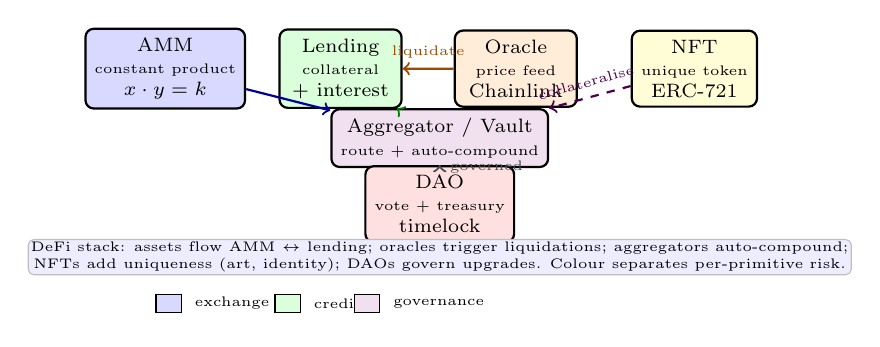
\begin{tikzpicture}[scale=0.84, every node/.style={font=\scriptsize},
  prim/.style={draw,rounded corners=3pt,minimum width=1.55cm,minimum height=0.62cm,align=center,thick}]
\node[prim,fill=blue!15] (amm) at (0,2.10) {AMM\\ \tiny constant product\\ $x\cdot y=k$};
\node[prim,fill=green!14] (lend) at (2.65,2.10) {Lending\\ \tiny collateral\\ + interest};
\node[prim,fill=orange!15] (oracle) at (5.30,2.10) {Oracle\\ \tiny price feed\\ Chainlink};
\node[prim,fill=yellow!16] (nft) at (8.00,2.10) {NFT\\ \tiny unique token\\ ERC-721};
\node[prim,fill=violet!12] (aggr) at (4.15,1.05) {Aggregator / Vault\\ \tiny route + auto-compound};
\node[prim,fill=red!12] (dao) at (4.15,0.05) {DAO\\ \tiny vote + treasury\\ timelock};
\draw[->,thick,blue!60!black] (amm)--(aggr); \draw[->,thick,green!50!black] (lend)--(aggr);
\draw[->,thick,orange!60!black] (oracle)--(lend) node[midway,above,font=\tiny,sloped] {liquidate};
\draw[->,thick,gray!60!black,dashed] (aggr)--(dao) node[midway,right,font=\tiny] {governed};
\draw[->,thick,violet!60!black,dashed] (nft)--(aggr) node[midway,above,font=\tiny,sloped] {collateralise};
% flow annotation
\node[font=\tiny,fill=blue!7,draw=gray!50,rounded corners=2pt,inner sep=1pt,align=center] at (4.15,-0.75) {DeFi stack: assets flow AMM $\leftrightarrow$ lending; oracles trigger liquidations; aggregators auto-compound;\\NFTs add uniqueness (art, identity); DAOs govern upgrades. Colour separates per-primitive risk.};
% legend
\node[draw,fill=blue!15,minimum width=0.32cm,minimum height=0.18cm] at (0.05,-1.45) {}; \node[font=\tiny,anchor=west] at (0.30,-1.45) {exchange};
\node[draw,fill=green!14,minimum width=0.32cm,minimum height=0.18cm] at (1.85,-1.45) {}; \node[font=\tiny,anchor=west] at (2.10,-1.45) {credit};
\node[draw,fill=violet!12,minimum width=0.32cm,minimum height=0.18cm] at (3.05,-1.45) {}; \node[font=\tiny,anchor=west] at (3.30,-1.45) {governance};
\end{tikzpicture}
\caption{Composable primitives: AMM for swapping, lending for leverage, oracles for external truth, NFTs for uniqueness, and DAOs for governance. Real apps (Uniswap, Aave, MakerDAO) are compositions, not singletons.}
\label{fig:defi-stack}
\end{figure}

\begin{example}[Constant-product AMM]\label{ex:amm}
Reserves $(x,y)$ with invariant $x\cdot y=k$. Swapping $\Delta x$ for $\Delta y$ gives $\Delta y = y - k/(x+\Delta x)$. Price impact grows with trade size; arbitrageurs restore $x/y$ to the external market price, paying fees to liquidity providers. Impermanent loss is the opportunity cost vs holding.
\end{example}

Other domains: \emph{supply chain} (provenance via tokenised batches plus ZK for privacy), \emph{identity} (verifiable credentials anchored on-chain), and \emph{gaming} (true ownership of in-game assets via NFTs plus on-chain logic).

% ============================================================
\section{Tokenomics: Designing Incentives}\label{sec:tokenomics}
A \emph{token} is a programmable unit of value/utility/governance. Good tokenomics answers: supply schedule, allocation, inflation, yield and value accrual.

\begin{definition}[Supply and emission]\label{def:supply}
\emph{Max supply} $S_{\max}$ is the cap; \emph{circulating} $S_t$ at time $t$ follows an \emph{emission curve} (e.g., Bitcoin halving: reward halves every 210\,k blocks). \emph{Inflation} $i_t=(S_{t+1}-S_t)/S_t$ funds security (staking rewards) but dilutes holders. \emph{Staking yield} $y_t$ pays stakers to lock capital; real yield $=y_t - i_t$ if all stake.
\end{definition}

\begin{figure}[h]\centering
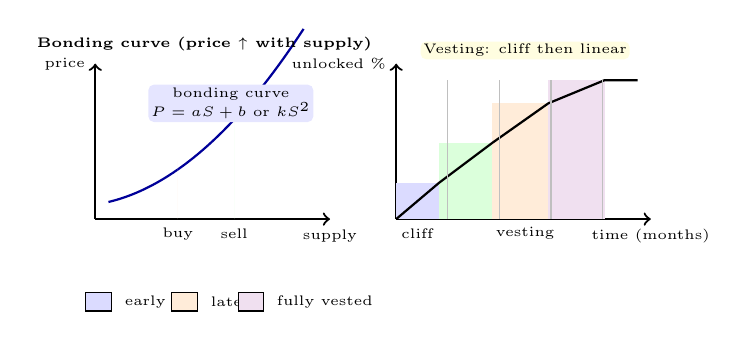
\begin{tikzpicture}[scale=0.84, every node/.style={font=\scriptsize}]
% bonding curve
\begin{scope}[xshift=0cm]
  \draw[->,thick] (0,0) -- (3.55,0) node[below,font=\tiny] {supply};
  \draw[->,thick] (0,0) -- (0,2.35) node[left,font=\tiny] {price};
  \draw[thick,blue!60!black,domain=0.20:3.15,smooth,samples=40] plot (\x,{0.22*\x*\x+0.15*\x+0.22});
  \node[font=\tiny,fill=blue!10,rounded corners=2pt,inner sep=1pt,align=center] at (2.05,1.75) {bonding curve\\ $P=aS+b$ or $kS^2$};
  \fill[orange!16] (1.25,0) rectangle (1.25,0.88); \fill[green!14] (2.10,0) rectangle (2.10,1.55);
  \node[font=\tiny] at (1.25,-0.22) {buy}; \node[font=\tiny] at (2.10,-0.22) {sell};
  \node[font=\tiny\bfseries] at (1.65,2.65) {Bonding curve (price $\uparrow$ with supply)};
\end{scope}
% vesting schedule
\begin{scope}[xshift=4.55cm]
  \draw[->,thick] (0,0) -- (3.85,0) node[below,font=\tiny] {time (months)};
  \draw[->,thick] (0,0) -- (0,2.35) node[left,font=\tiny] {unlocked \%};
  \fill[blue!14] (0,0) rectangle (0.65,0.55);
  \fill[green!14] (0.65,0) rectangle (1.45,1.15);
  \fill[orange!15] (1.45,0) rectangle (2.30,1.75);
  \fill[violet!12] (2.30,0) rectangle (3.15,2.10);
  \draw[thick] (0,0) -- (0.65,0.55) -- (1.45,1.15) -- (2.30,1.75) -- (3.15,2.10) -- (3.65,2.10);
  \foreach \m/\p in {6/25,12/50,18/75,24/100} \draw[thin,gray!50] (\m*0.13,0) -- (\m*0.13,2.10);
  \node[font=\tiny,fill=yellow!12,rounded corners=2pt,inner sep=1pt] at (1.95,2.55) {Vesting: cliff then linear};
  \node[font=\tiny] at (0.32,-0.22) {cliff}; \node[font=\tiny] at (1.95,-0.22) {vesting};
\end{scope}
% legend
\node[draw,fill=blue!14,minimum width=0.32cm,minimum height=0.18cm] at (0.05,-1.25) {}; \node[font=\tiny,anchor=west] at (0.30,-1.25) {early};
\node[draw,fill=orange!15,minimum width=0.32cm,minimum height=0.18cm] at (1.35,-1.25) {}; \node[font=\tiny,anchor=west] at (1.60,-1.25) {later};
\node[draw,fill=violet!12,minimum width=0.32cm,minimum height=0.18cm] at (2.35,-1.25) {}; \node[font=\tiny,anchor=west] at (2.60,-1.25) {fully vested};
\end{tikzpicture}
\caption{Left: bonding curve (price as function of supply) for continuous token offerings. Right: vesting schedule (cliff + linear) to align long-term incentives. Colour tracks time/price progression.}
\label{fig:tokenomics}
\end{figure}

A \emph{bonding curve} $P(S)$ sets price by supply (e.g., $P=aS$), enabling permissionless issuance. \emph{Vesting} (cliff then linear unlock) prevents early dumps. Key tensions: high inflation secures the chain but dilutes; deflationary burns (EIP-1559) help holders but may underpay security.

\begin{lstlisting}[language=Python]
# AMM constant-product swap + bonding curve pricer
def amm_swap(x,y, dx):
    k=x*y
    dy = y - k/(x+dx)
    return dy, x+dx, y-dy

x,y=100000, 100000  # reserves
for sz in [100,1000,5000,10000]:
    dy,_,_=amm_swap(x,y, sz)
    price = dy/sz
    print(f"swap {sz}: get {round(dy,1)}, avg price {round(price,4)} (slippage up)")
# Bonding curve linear: P = 0.01*S + 1, cost to mint dS = integral P dS
def bonding_cost(S, dS, a=0.01, b=1.0):
    # integral of a*s+b ds from S to S+dS
    return 0.5*a*((S+dS)**2 - S**2) + b*dS
print("mint 100 at S=1000:", round(bonding_cost(1000,100),2))
# Vesting
def vested(t, cliff=6, total=24):
    if t < cliff: return 0.0
    return min(1.0, (t-cliff)/(total-cliff))
for m in [0,6,12,18,24]:
    print(f"month {m}: {vested(m)*100:.0f}% unlocked")
\end{lstlisting}

% ============================================================
\section{Governance, DAOs and Trade-offs}\label{sec:governance}
Code needs upgrades and treasuries need spending; \emph{governance} decides how. On-chain governance token vote $\to$ timelock $\to$ execute is the DAO pattern, but it faces plutocracy (whales dominate), voter apathy, and vote-buying/bribery (MEV of governance).

\begin{figure}[h]\centering
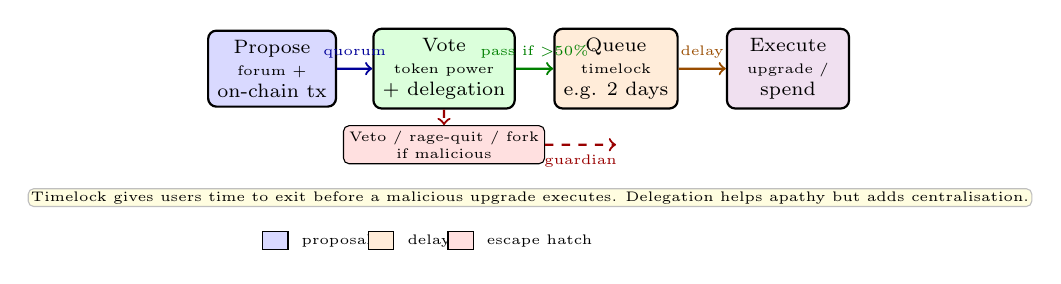
\begin{tikzpicture}[scale=0.84, every node/.style={font=\scriptsize},
  mystep/.style={draw,rounded corners=3pt,minimum width=1.55cm,minimum height=0.65cm,align=center,thick}]
\node[mystep,fill=blue!15] (prop) at (0,1.70) {Propose\\ \tiny forum +\\ on-chain tx};
\node[mystep,fill=green!14] (vote) at (2.60,1.70) {Vote\\ \tiny token power\\ + delegation};
\node[mystep,fill=orange!15] (queue) at (5.20,1.70) {Queue\\ \tiny timelock\\ e.g. 2 days};
\node[mystep,fill=violet!12] (exec) at (7.80,1.70) {Execute\\ \tiny upgrade /\\ spend};
\draw[->,thick,blue!60!black] (prop)--(vote) node[midway,above,font=\tiny] {quorum};
\draw[->,thick,green!50!black] (vote)--(queue) node[midway,above,font=\tiny] {pass if >50\%};
\draw[->,thick,orange!60!black] (queue)--(exec) node[midway,above,font=\tiny] {delay};
\node[draw,fill=red!12,rounded corners=2pt,inner sep=2pt,font=\tiny,align=center] (veto) at (2.60,0.55) {Veto / rage-quit / fork\\ if malicious};
\draw[->,thick,red!60!black,dashed] (vote) -- (veto);
\draw[->,thick,red!60!black,dashed] (veto) -- (5.20,0.55) node[midway,below,font=\tiny] {guardian};
\node[font=\tiny,fill=yellow!12,draw=gray!50,rounded corners=2pt,inner sep=1pt,align=center] at (3.90,-0.25) {Timelock gives users time to exit before a malicious upgrade executes. Delegation helps apathy but adds centralisation.};
% legend
\node[draw,fill=blue!15,minimum width=0.32cm,minimum height=0.18cm] at (0.05,-0.90) {}; \node[font=\tiny,anchor=west] at (0.30,-0.90) {proposal};
\node[draw,fill=orange!15,minimum width=0.32cm,minimum height=0.18cm] at (1.65,-0.90) {}; \node[font=\tiny,anchor=west] at (1.90,-0.90) {delay};
\node[draw,fill=red!12,minimum width=0.32cm,minimum height=0.18cm] at (2.85,-0.90) {}; \node[font=\tiny,anchor=west] at (3.10,-0.90) {escape hatch};
\end{tikzpicture}
\caption{DAO governance lifecycle: proposal $\to$ vote (with delegation) $\to$ timelocked queue $\to$ execution. Red shows escape hatches (veto, rage-quit, fork) when governance is captured.}
\label{fig:dao}
\end{figure}

\begin{remark}[Decentralisation spectrum]\label{rem:spectrum}
``Decentralised'' is not binary: count clients, operators, geographic spread, and governance concentration. A chain with one dominant client, three validators and whale-controlled governance is technically a blockchain but not meaningfully decentralised. Regulation adds another axis: privacy (ZK, mixers) vs compliance (KYC at on/off-ramps, travel rule).
\end{remark}

\begin{example}[So you want to build a token?]\label{ex:token-recipe}
Checklist before writing code: (1) what is scarce and why should it be on-chain rather than in a database? (2) who must hold the token for the system to function (users, stakers, LPs)? (3) what sinks/burns offset emissions? (4) how does governance upgrade the system without capture? If you cannot answer all four, you may not need a token -- a common lesson in the 2022 crash.
\end{example}

\begin{remark}[Regulation and the road ahead]\label{rem:regulation}
Regulators increasingly treat tokens as securities, stablecoins as e-money, and mixers as money-transmission. Designing for compliance (allow-listed pools, view keys, audit trails) versus maximal privacy is now a product decision with legal consequences. The technology of Ch.~1--7 is neutral; the deployment is not.
\end{remark}

\begin{example}[Reading a whitepaper]\label{ex:whitepaper}
When assessing a new chain, ask: (1) what is the Sybil-resistance mechanism and its cost to attack? (2) what is the light-client proof size? (3) where is data availability posted and at what cost? (4) what is the formal spec for the token's monetary policy? Vague answers to any of these are red flags.
\end{example}

\begin{lstlisting}[language=Python]
# DAO voting + timelock simulator
from collections import defaultdict
votes = defaultdict(int)  # choice -> power
# delegation: Alice delegates to Bob
deleg = {"Alice": "Bob"}
power = {"Bob": 60, "Carol": 40, "Dave": 15}  # Bob includes Alice's 10
# tally
for voter, p in power.items():
    votes["yes"] += p if voter in ["Bob","Carol"] else 0
    votes["no"]  += p if voter=="Dave" else 0
print("tally", dict(votes), "pass?" , votes["yes"] > votes["no"])
# timelock: proposal queued at t=0, executable after delay
delay=2  # days
for t in [0,1,2,3]:
    print(f"day {t}: {'executable' if t>=delay else 'timelocked'}")
# Bonding outcome after DAO spend
treasury=1_000_000
spend=200_000
print("treasury after spend:", treasury-spend)
\end{lstlisting}

% ============================================================
\section{Exercises}\label{sec:ch08-exercises}
\begin{enumerate}[label=E8.\arabic*, leftmargin=*, itemsep=0.6em]
    \item \textbf{AMM slippage.} Reserves $(100k,100k)$, $k=10^{10}$. Compute output and average price for swaps $1k,10k,50k$. Plot slippage vs size. At what size does price deviate 5\% from spot?
    \item \textbf{Emission design.} Design a 4-year halving schedule from 50 to 3.125 per block for 10\,min blocks. Compute total supply after 4 halvings and annual inflation each year.
    \item \textbf{Vesting game.} Team gets 20\% with 1-year cliff + 3-year linear vest. Investor gets 10\% with 6-month cliff + 1-year linear. Sketch both curves and argue who can dump first and the market impact.
    \item \textbf{Governance attack.} An attacker flash-loans governance tokens, votes, and repays in one block. Explain why snapshot-at-proposal-start and timelock mitigate this. Propose a vote-escrow (veToken) alternative.
    \item \textbf{Whitepaper critique.} Pick any live project's whitepaper claims (throughput, decentralisation, tokenomics). Map each claim to a Ch.~2/5/6/7 check (consensus proof, Merkle cost, rollup data, MEV) and flag one unsubstantiated statement.
\end{enumerate}

\section*{Chapter Notes}
Buterin (2013) whitepaper and Wood (Yellow Paper) for app/token foundations; Adams et al., Uniswap v2/v3 for AMMs; EIP-1559 and tokenomics surveys (Messari, 2022) for supply design; DAO governance and bribery in Daian--Goldfeder analyses and Optimism Collective docs. Narayanan et al., Ch.~9--10 for the application landscape; Bonneau et al., SoK on cryptocurrencies (2015) for the research map.
% End Ch08
